% 113-77(113쪽) — 함수 y=f(t) 의 그래프(t 축을 O 왼쪽·2·4 에서 지나는 삼차 모양). 스캔 화질이 낮아 TikZ 로 다시 그림.
% 원문에 있는 것만: t 축 눈금 2 와 4 · 라벨 O, t, y, y=f(t). y 눈금·극값 좌표는 원문에 없으므로 넣지 않는다
% (정적분 값이 발문에 주어져 있고 최댓값·최솟값이 답이라 그림에서 수치가 읽히면 안 된다).
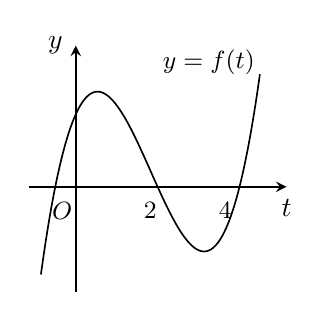
\begin{tikzpicture}[x=0.52cm, y=0.46cm, line width=0.5pt]
  \draw[->, >=stealth, line width=0.7pt] (-1.15,0) -- (5.15,0) node[below=1pt] {$t$};
  \draw[->, >=stealth, line width=0.7pt] (0,-2.9) -- (0,3.9) node[left=1pt] {$y$};
  \node[below=2pt, font=\small] at (-0.33,0) {$\pt{O}$};
  % 그래프 — t=-0.5, 2, 4 에서 t 축을 지나는 모양(원문 그대로)
  \draw[line width=0.6pt, domain=-0.85:4.5, samples=180, smooth] plot (\x, {0.5*(\x+0.5)*(\x-2)*(\x-4)});
  \node[below=2pt, font=\small] at (1.82,0) {$2$};
  \node[below=2pt, font=\small] at (3.65,0) {$4$};
  \node[font=\small] at (3.25,3.45) {$y=f(t)$};
\end{tikzpicture}
